\section{Results}
In our experiments we answer the following questions:
\begin{description}
	\item[Q1] How does the performance of DL8.5 compare to DL8, MIP-based and CP-based approaches on binary data?
	\item[Q2] What is the impac\emph{TO}f different branching heuristics on the performance of DL8.5?
	\item[Q3] What is the impac\emph{TO}f caching incomplete results in DL8.5 (NO TREE itemsets)?
	\item[Q4] How does the performance of DL8.5 compare to DL8, MIP-based and CP-based approaches on continuous data?
\end{description}
As a representative MIP-based approach, we use BinOCT, as it was shown to be the best performing MIP-based approach in a recent study (Verwer and Zhang 2019). The implementations of BinOCT\footnote{https://github.com/SiccoVerwer/binoct}, DL8 and the CP-based approach\footnote{https://bitbucket.org/helene\_verhaeghe/classificationtree/src/ default/classificationtree/} used in our comparison were obtained from their original authors, and use the CPLEX 12.9\footnote{https://www.ibm.com/analytics/cplex-optimizer} and OscaR\footnote{https://oscarlib.bitbucket.io} solvers. Experiments were performed on a server with an Intel Xeon E5-2640 CPU, 128GB of memory, running Red Hat 4.8.5-16.

To respect the constrain\emph{TO}f the CP-based algorithm all the datasets used in our experiments have binary classes. We compare our algorithms on 24 binary datasets from CP4IM\footnote{https://dtai.cs.kuleuven.be/CP4IM/datasets/}, described in the first columns of Table \ref{tab:2}.

Similar to Verwer and Zhang (2019), we run the different algorithms for 10 minutes on each dataset and for a maximum depth of 2, 3 and 4. All the tests are run with a minimum suppor\emph{TO}f 1 since this is the setting used in BinOCT.

We do not spli\emph{TO}ur datasets in training and test sets since the focus of this work is on comparing the computational performance of algorithms that should generate decision trees of the same quality. The benefits of optimal decision trees were discussed in (Bertsimas and Dunn 2017).

We compare a number of variants of DL8.5. The following table summarizes the abbreviations used.

\noindent\begin{tabularx}{\linewidth}{lX}
	Abbreviation	& Meaning		\\\hline
	d.o.			& the original order of the attributes in the data is used as branching heuristic		\\
	asc				& attributes are sorted in increasing value of information gain		\\
	desc			& attributes are sorted in decreasing value of information gain		\\
	n.p.s.			& no partial solutions are stored in the cache
\end{tabularx}

Table \ref{tab:2} shows the results for a maximum depth equal to 4, as we consider deeper decision trees of more interest. If optimality could not be proven within 10 minutes, this is indicated using \emph{TO}; in this case, the objective value of the best tree found so far is shown. Note that we here exploit the ability of DL8.5 to produce a result after a time-out. The best solutions and best times are marked in bold while a star (*) is added to mark solutions proven to be optimal.

BinOCT solved and proved optimality for only 1 instance within the timeout; the older DL8 algorithm solved 7 instances and the CP-based algorithm solved 11 instances. DL8.5 solved 19 (which answers \textbf{Q1}). The difference in performance is further illustrated in Figure \ref{fig:4}, which gives \emph{cactus plots} for each algorithm, for different depth constraints. In these plots each point $(x, y)$ indicates the number of instances $(x)$ solved within a time limit $(y)$. While for lower depth thresholds, BinOCT does find solutions, the performance of all variants of DL8.5 clearly remains superior to tha\emph{TO}f DL8, BinOCT and the CP-based algorithm, obtaining orders of magnitude better performance.

Comparing the different branching heuristics in DL8.5, the differences are relatively small; however, for deeper trees, a descending order of information gain gives slightly better results. This confirms the intuition that chosen a split with high information gain is a good heuristic (\textbf{Q2}).

If we disable DL8.5’s ability to cache incomplete results, we see a significant degradation in performance. In this varian\emph{TO}nly 12 instances are solved optimally, instead of 19, for a depth of 4. Hence, this optimization is significant (\textbf{Q3}).

To answer \textbf{Q4}, we repeat these tests on continuous data. For this, we use the same datasets as Verwer and Zhang (2019). These datasets were obtained from the UCI repository\footnote{https://archive.ics.uci.edu/ml/index.php} and are summarized in the first columns of Table \ref{tab:3}. Before running DL8, the CP-based algorithm and DL8.5, we binarize these datasets by creating binary features using the same approach as the one used by Verwer and Zhang (2019). Note that the number of generated features is very high in this case. As a result, for most datasets all algorithms reach a time-out for maximum depths of 3 and 4, as was also shown by Verwer and Zhang (2019). Hence, we focus on results for a depth of 2 in Table \ref{tab:3}. Even though BinOCT uses a specialized technique for solving continuous data, the table shows that DL8.5 outperforms DL8, the CP-based algorithm and BinOCT. Note that the differences between the different variations of DL8.5 are small here, which may not be surprising given the shallowness of the search tree considered.

\begin{table*}
	\tiny\centering
	\begin{tabular}{|L{0.08\linewidth}|*{10}{C{0.03\linewidth}|}|*{2}{C{0.03\linewidth}|}|*{2}{C{0.03\linewidth}|}|*{2}{C{0.03\linewidth}|}}
		\hline
		\multirow{3}{*}{Dataset}	& \multirow{3}{*}{nItems}	 & \multirow{3}{*}{nTrans}	& \multicolumn{2}{c|}{BinOCT} &\multicolumn{2}{c|}{DL8}	&\multicolumn{2}{c|}{CP-Based}	& \multicolumn{8}{c|}{DL8.5}		\\
		& 	 & 	& & &&	&&	& \multicolumn{2}{c||}{d.o.}	& \multicolumn{2}{c||}{asc}	& \multicolumn{2}{c||}{desc}	& \multicolumn{2}{c|}{n.p.s.}		\\
		& 	 & 	& \rotatebox{90}{obj} & \rotatebox{90}{time (s)} & \rotatebox{90}{obj}& \rotatebox{90}{time (s)}	& \rotatebox{90}{obj}	& \rotatebox{90}{time (s)}	& \rotatebox{90}{obj}	& \rotatebox{90}{time (s)}	& \rotatebox{90}{obj}	& \rotatebox{90}{time (s)}	& \rotatebox{90}{obj}	& \rotatebox{90}{time (s)}	&\rotatebox{90}{obj}	& \rotatebox{90}{time (s)}	\\
		\hline\hline
		anneal	& 186 	& 812	& 115	& $TO$	& $\infty$	& $TO$	&\bf 91*	&\bf 450.69	&\bf 91*	& 129.24	&\bf 91*	& 127.45	&\bf 91*	& 121.87	& 91*	& 250.64		\\
		\hline
		audiology	& 296	& 216	& 2	& \emph{TO}	& $\infty$	& \emph{TO}	& 1	& \emph{TO}	& 1*	& 180.84	& 1*	& 204.19	& 1*	& 195.73	& 1	& \emph{TO}		\\
		\hline
		australian-credit	& 250	& 653	& 82	& \emph{TO}	& $\infty$	& \emph{TO}	& 66	& \emph{TO}	&\bf 56*	& 566.71	&\bf 56*	& 586.39	&\bf 56*	& 593.38	& 57	& \emph{TO}		\\
		\hline
		breast-wisconsin	& 240	& 683	& 12	& \emph{TO}	& $\infty$	& \emph{TO}	& 8	& \emph{TO}	&\bf 7*	& 305.3	&\bf 7*	& 325.7	&\bf 7*	& 330.71	& 7	& \emph{TO}		\\
		\hline
		diabetes	& 224	& 768	& 170	& \emph{TO}	& $\infty$	& \emph{TO}	& 140	& \emph{TO}	&\bf 137*	& 553.49	&\bf 137*	& 562.83	&\bf 137*	& 565.5	& 137	& \emph{TO}			\\
		\hline
		german-credit	& 224	& 1000	& 223	& \emph{TO}	& $\infty$	& \emph{TO}	& 204	& \emph{TO}	&\bf 204*	& 558.73	& 206	& \emph{TO}	&\bf 204*	& 599.87	& 204	& \emph{TO}		\\
		\hline
		heart-cleveland	& 190	& 296	& 39	& \emph{TO}	& $\infty$	& \emph{TO}	& 25	& \emph{TO}	&\bf 25*	& 124.1	&\bf 25*	& 130.3	&\bf 25*	& 132.23	&\bf 25*	& 214.76	    \\
		\hline
		hepatitis	& 136	& 137	& 7	& \emph{TO}	&\bf 3*	& 66.62	&\bf 3*	& 109.36	& \bf 3*	& 13.46	& \bf 3*	& 14.06	& \bf 3*	& 14.88	& \bf 3*	& 27.28         \\
		\hline
		hypothyroid	& 176	& 3247	& 55	& \emph{TO}	& $\infty$	& \emph{TO}	& 53	& \emph{TO}	&\bf 53*	& 392.22	&\bf 53*	& 368.95	&\bf 53*	& 427.34	& 53	& \emph{TO}	    \\
		\hline
		ionosphere	& 890	& 351	& 27	& \emph{TO}	& $\infty$	& \emph{TO}	& 20	& \emph{TO}	& 17	& \emph{TO}	& 11	& \emph{TO}	& 13	& \emph{TO}	& 17	& \emph{TO}       \\
		\hline
		kr-vs-kp	& 146	& 3196	& 193	& \emph{TO}	& $\infty$	& \emph{TO}	&\bf 144*	& 483.15	&\bf 144*	& 216.11	&\bf 144*	& 206.18	&\bf 144*	& 223.85	&\bf 144*	& 528.72        \\
		\hline
		letter	& 448	& 20000	& 813	& \emph{TO}	& $\infty$	& \emph{TO}	& 574	& \emph{TO}	& 550	& \emph{TO}	& 586	& \emph{TO}	& 802	& \emph{TO}	& 550	& \emph{TO}       \\
		\hline
		lymph	& 136	& 148	& 6	& \emph{TO}	&\bf 3*	& 56.29	&\bf 3*	& 112.48	&\bf 3*	& 8.7	&\bf 3*	& 11.03	&\bf 3*	& 8.47	&\bf 3*	& 25.04     \\\hline
		mushroom	& 238	& 8124	& 278	& \emph{TO}	& $\infty$	& \emph{TO}	&\bf 0*	& 352.18	&\bf 0*	& 331.39	& 4	& \emph{TO}	&\bf 0*	& 0.11	& 4	& \emph{TO}	    \\
		\hline
		pendigits	& 432	& 7494	& 780	& \emph{TO}	& $\infty$	& \emph{TO}	& 38	& \emph{TO}	& 32	& \emph{TO}	& 26	& \emph{TO}	& 14	& \emph{TO}	& 32	& \emph{TO}       \\
		\hline
		primary-tumor	& 62	& 336	& 37	& \emph{TO}	&\bf 34*	& 2.79	&\bf 34*	& 8.96	&\bf 34*	& 1.48	& \bf34*	& 1.51	& 34*	& 1.38	&\bf 34*	& 2.43      \\
		\hline
		segment	& 470	& 2310	& 13	& \emph{TO}	& $\infty$	& \emph{TO}	&\bf 0*	& 128.25	&\bf 0*	& 3.54	&\bf 0*	& 6.99	&\bf 0*	& 7.05	&\bf 0*	& 3.54      \\
		\hline
		soybean	& 100	& 630	& 15	& \emph{TO}	&\bf 14*	& 41.59	&\bf 14*	& 40.13	&\bf 14*	& 5.7	&\bf 14*	& 6.34	&\bf 14*	& 5.75	&\bf 14*	& 18.41     \\
		\hline
		splice-1	& 574	& 319	& 574	& \emph{TO}	& $\infty$	& \emph{TO}	& $\infty$	& \emph{TO}	& 224	& \emph{TO}	& 224	& \emph{TO}	& 141	& \emph{TO}	& 224	& \emph{TO}       \\
		\hline
		tic-tac-toe	& 54	& 958	& 180	& \emph{TO}	&\bf 137*	& 3.76	&\bf 137*	& 9.17	&\bf 137*	& 1.43	&\bf 137*	& 1.54	&\bf 137*	& 1.55	&\bf 137*	& 2.12      \\
		\hline
		vehicle	& 504	& 846	& 61	& \emph{TO}	& $\infty$	& \emph{TO}	& 22	& \emph{TO}	& 16	& \emph{TO}	& 18	& \emph{TO}	& 13	& \emph{TO}	& 16	& \emph{TO}       \\
		\hline
		vote	& 96	& 435	& 6	& \emph{TO}	&\bf 5*	& 29.84	&\bf 5*	& 44.47	&\bf 5*	& 5.48	&\bf 5*	& 5.33	&\bf 5*	& 5.58	&\bf 5*	& 12.82     \\
		\hline
		yeast	& 178	& 1484	& 395	& \emph{TO}	& $\infty$	& \emph{TO}	& 366	& \emph{TO}	&\bf 366*	& 318.87	&\bf 366*	& 326.2	&\bf 366*	& 334.15	&\bf 366*	& 470.88        \\
		\hline
		zoo-1	& 72	& 101	&\bf 0*	& 0.52	&\bf 0*	& 1.11	&\bf 0*	& 0.2	&\bf 0*	& 0.01	&\bf 0*	& 0.01	&\bf 0*	& 0.01	&\bf 0*	& 0.01      \\
		\hline
	\end{tabular}
	\caption{: Comparison table for binary datasets with max depth = 4}
	\label{tab:2}
\end{table*}
\begin{figure*}
	\centering
	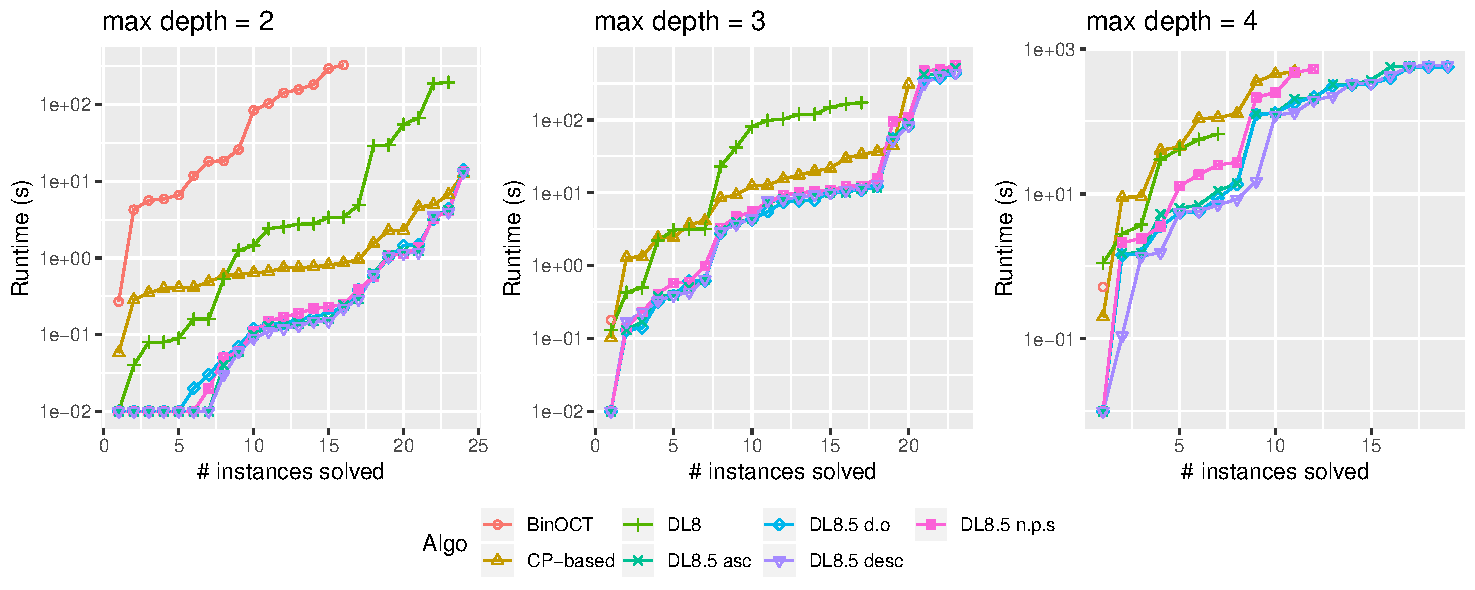
\includegraphics[width=0.9\linewidth]{cactus_log}
	\caption{Cumulative number of instances solved over time}
	\label{fig:4}
\end{figure*}
\begin{table*}
	\tiny\centering
	\begin{tabular}{|L{0.08\linewidth}|*{11}{C{0.03\linewidth}|}|*{2}{C{0.03\linewidth}|}|*{2}{C{0.03\linewidth}|}}
		\hline
		\multirow{3}{*}{Dataset}	& \multirow{3}{*}{nTrans}	 & \multirow{3}{*}{nFeat}	& \multirow{3}{*}{nItems}	& \multicolumn{2}{c|}{BinOCT} &\multicolumn{2}{c|}{DL8}	&\multicolumn{2}{c|}{CP-Based}	& \multicolumn{6}{c|}{DL8.5}		\\
		& 	 & 	& & &&	&&	&& \multicolumn{2}{c||}{d.o.}	& \multicolumn{2}{c||}{asc}	& \multicolumn{2}{c||}{desc}		\\
			& 	 & 	&& \rotatebox{90}{obj} & \rotatebox{90}{time (s)} & \rotatebox{90}{obj}& \rotatebox{90}{time (s)}	& \rotatebox{90}{obj}	& \rotatebox{90}{time (s)}	& \rotatebox{90}{obj}	& \rotatebox{90}{time (s)}	& \rotatebox{90}{obj}	& \rotatebox{90}{time (s)}	& \rotatebox{90}{obj}	& \rotatebox{90}{time (s)}		\\
		\hline\hline
		balance-scale   & 625   & 4 & 32  & \bf 149* & 1.2 & \bf 149*    & 0.5    & \bf 149*   & 0.01  & \bf 149* & 0.01    & \bf 149*   & 0.01  & \bf 149* & 0.01\\
		\hline
		banknote  & 1372  & 4	& 3710  & 101  & \emph{TO}  & \bf 100*  & 363.01  & $\infty$  & \emph{TO}  & \bf 100*  & 52.81  & \bf 100*  & 63.41  & \bf 100*  & 58.07\\
		\hline
		bank  & 4521  & 51  & 3380  & 449  & \emph{TO}  & 448  & \emph{TO}  & $\infty$  & \emph{TO}  & \bf 44\bf 6*  & 253.87  & \bf 44\bf 6*  & 223.42  & \bf 44\bf 6*  & 222.66\\
		\hline
		biodeg  & 1055  & 41  & 8356  & 212  & \emph{TO}  & 212  & \emph{TO}  & $\infty$  & \emph{TO}  & \bf 202*  & 341.57  & \bf 202*  & 365.83  & \bf 202*  & 370.26\\
		\hline
		car  & 1728  & 6  & 28   & \bf 250*  & 4.09  & \bf 250*  & 0.32  & \bf 250*  & 0.02  & \bf 250*  & 0.01  & \bf 250*  & 0.01  & \bf 250*  & 0.01\\
		\hline
		IndiansDiabetes  & 768  & 8  & 1714  & 171  & \emph{TO}  & \bf 171*  & 36.75  & $\infty$  & \emph{TO}  & \bf 171*  & 7.43  & \bf 171*  & 8.46  & \bf 171*  & 8.72\\
		\hline
		Ionosphere  & 351  & 34  & 4624  & 29  & \emph{TO}  & \bf 29*  & 423.52  & $\infty$   & \emph{TO}  & \bf 29*  & 25.68  & \bf 29*  & 33.76  & \bf 29*  & 33.04\\
		\hline
		iris  & 150  & 4  & 52  & \bf 0*  & 0.02  & \bf 0*  & 0.05  & \bf 0*  & 0.01  & \bf 0*  & 0.01  & \bf 0*  & 0.01  & \bf 0*  & 0.01\\
		\hline
		letter    & 20000    & 16    & 352    & 625    & \emph{TO}    & \bf 591*    & 5.97    & \bf 591*    & 392.09    & \bf  591*    & 8.61    & \bf 591*    & 8.26    & \bf 591*    & 8.83\\
		\hline
		messidor    & 1151    & 19    & 9460    & 383    & \emph{TO}    & 383    & \emph{TO}    & $\infty$    & \emph{TO}    & 383*    & 533.27    & 383*    & 563.83    & 383*    & 534.32\\
		\hline
		monk1    & 124    & 6    & 22    & 22*    & 0.33    & 22*    & 0.28    & 22*    & 0.01    & 22*    & 0.01    & 22*    & 0.01    & 22*    & 0.01\\
		\hline
		monk2    & 169    & 6    & 22    & 57*    & 0.79    & 57*    & 0.28    & 57*    & 0.01    & 57*    & 0.01    & 57*    & 0.01    & 57*    & 0.01\\
		\hline
		monk3    & 122    & 6    & 22    & 8*    & 0.31    & 8*    & 0.28    & 8*    & 0.01    & 8*    & 0.01    & 8*    & 0.01    & 8*    & 0.01\\
		\hline
		seismic    & 2584    & 18    & 2240    & 166    & \emph{TO}    & 164*    & 117.34    & $\infty$    & \emph{TO}    & 164*    & 44.3    & 164*    & 47.36    & 164*    & 47.17\\
		\hline
		spambase    & 4601    & 57    & 16012    & 660    & \emph{TO}    & 900    & \emph{TO}    & $\infty$    & \emph{TO}    & 741    & \emph{TO}    & 845    & \emph{TO}    & 586    & \emph{TO}\\
		\hline
		Statlog    & 4435    & 36    & 3274    & 460    & \emph{TO}    & 443    & \emph{TO}    & $\infty$    & \emph{TO}    & 443*    & 205.14    & 443*    & 193.87    & 443*    & 188.9\\
		\hline
		tic-tac-toe    & 958    & 18    & 36    & 282*    & 7.52    & 282*    & 0.33    & 282*    & 0.01    & 282*    & 0.01    & 282*    & 0.01    & 282*    & 0.01\\
		\hline
		wine    & 178    & 13    & 1198    & 6*    & 73.1    & 6*    & 7.0    & 6*    & 74.72    & 6*    & 1.17    & 6*    & 1.45    & 6*    & 1.09\\
		\hline
	\end{tabular}
	\caption{ Comparison table for continuous datasets with max depth = 2}
	\label{tab:3}
\end{table*}